Hauptmenü anzeigen

FA-C \ref{c-menu} %FA-C 21 Hauptmenü

Anwendung beenden

FA-C \ref{c-menu} %FA-C 21 Hauptmenü

Zur Lobby-Übersicht wechseln

FA-C \ref{c-menu} %FA-C 21 Hauptmenü
FA-C \ref{c-lobby-overview} %FA-C 22 Lobby-Übersicht

Lobby-Übersicht anzeigen

FA-C \ref{c-lobby-overview} %FA-C 22 Lobby-Übersicht

Lobby-Übersicht verlassen

FA-C \ref{c-menu} %FA-C 21 Hauptmenü
FA-C \ref{c-lobby-overview} %FA-C 22 Lobby-Übersicht

Nutzernamen festlegen

FA-C \ref{c-username} %FA-C 26 Nutzername

Lobby erstellen

Konfigurationsdateien festlegen

FA-S \ref{c-partieconfig} %FA-S 1 Partie Konfiguration
FA-S \ref{c-szenarioconfig} %FA-S 2 Szenario Konfiguration
FA-S \ref{c-charakterconfig} %FA-S 3 Charakter Konfiguration

Lobby beitreten

FA-C \ref{c-join} %FA-C 23 Beitreten als Mitspieler
FA-C \ref{c-join-spectator} %FA-C 24 Beitreten als Zuschauer
FA-S \ref{c-zuschauer} %FA-S 5 Zuschauer

Lobby anzeigen

Lobby verlassen

FA-C \ref{c-lobby-overview} %FA-C 22 Lobby-Übersicht

Rolle wechseln

FA-C \ref{c-join} %FA-C 23 Beitreten als Mitspieler
FA-C \ref{c-join-spectator} %FA-C 24 Beitreten als Zuschauer
FA-S \ref{c-zuschauer} %FA-S 5 Zuschauer

Spiel starten
FA-S \ref{c-partieinit} %FA-S 8 Spiel Start und Initialisierung


\begin{figure}
  \centering
  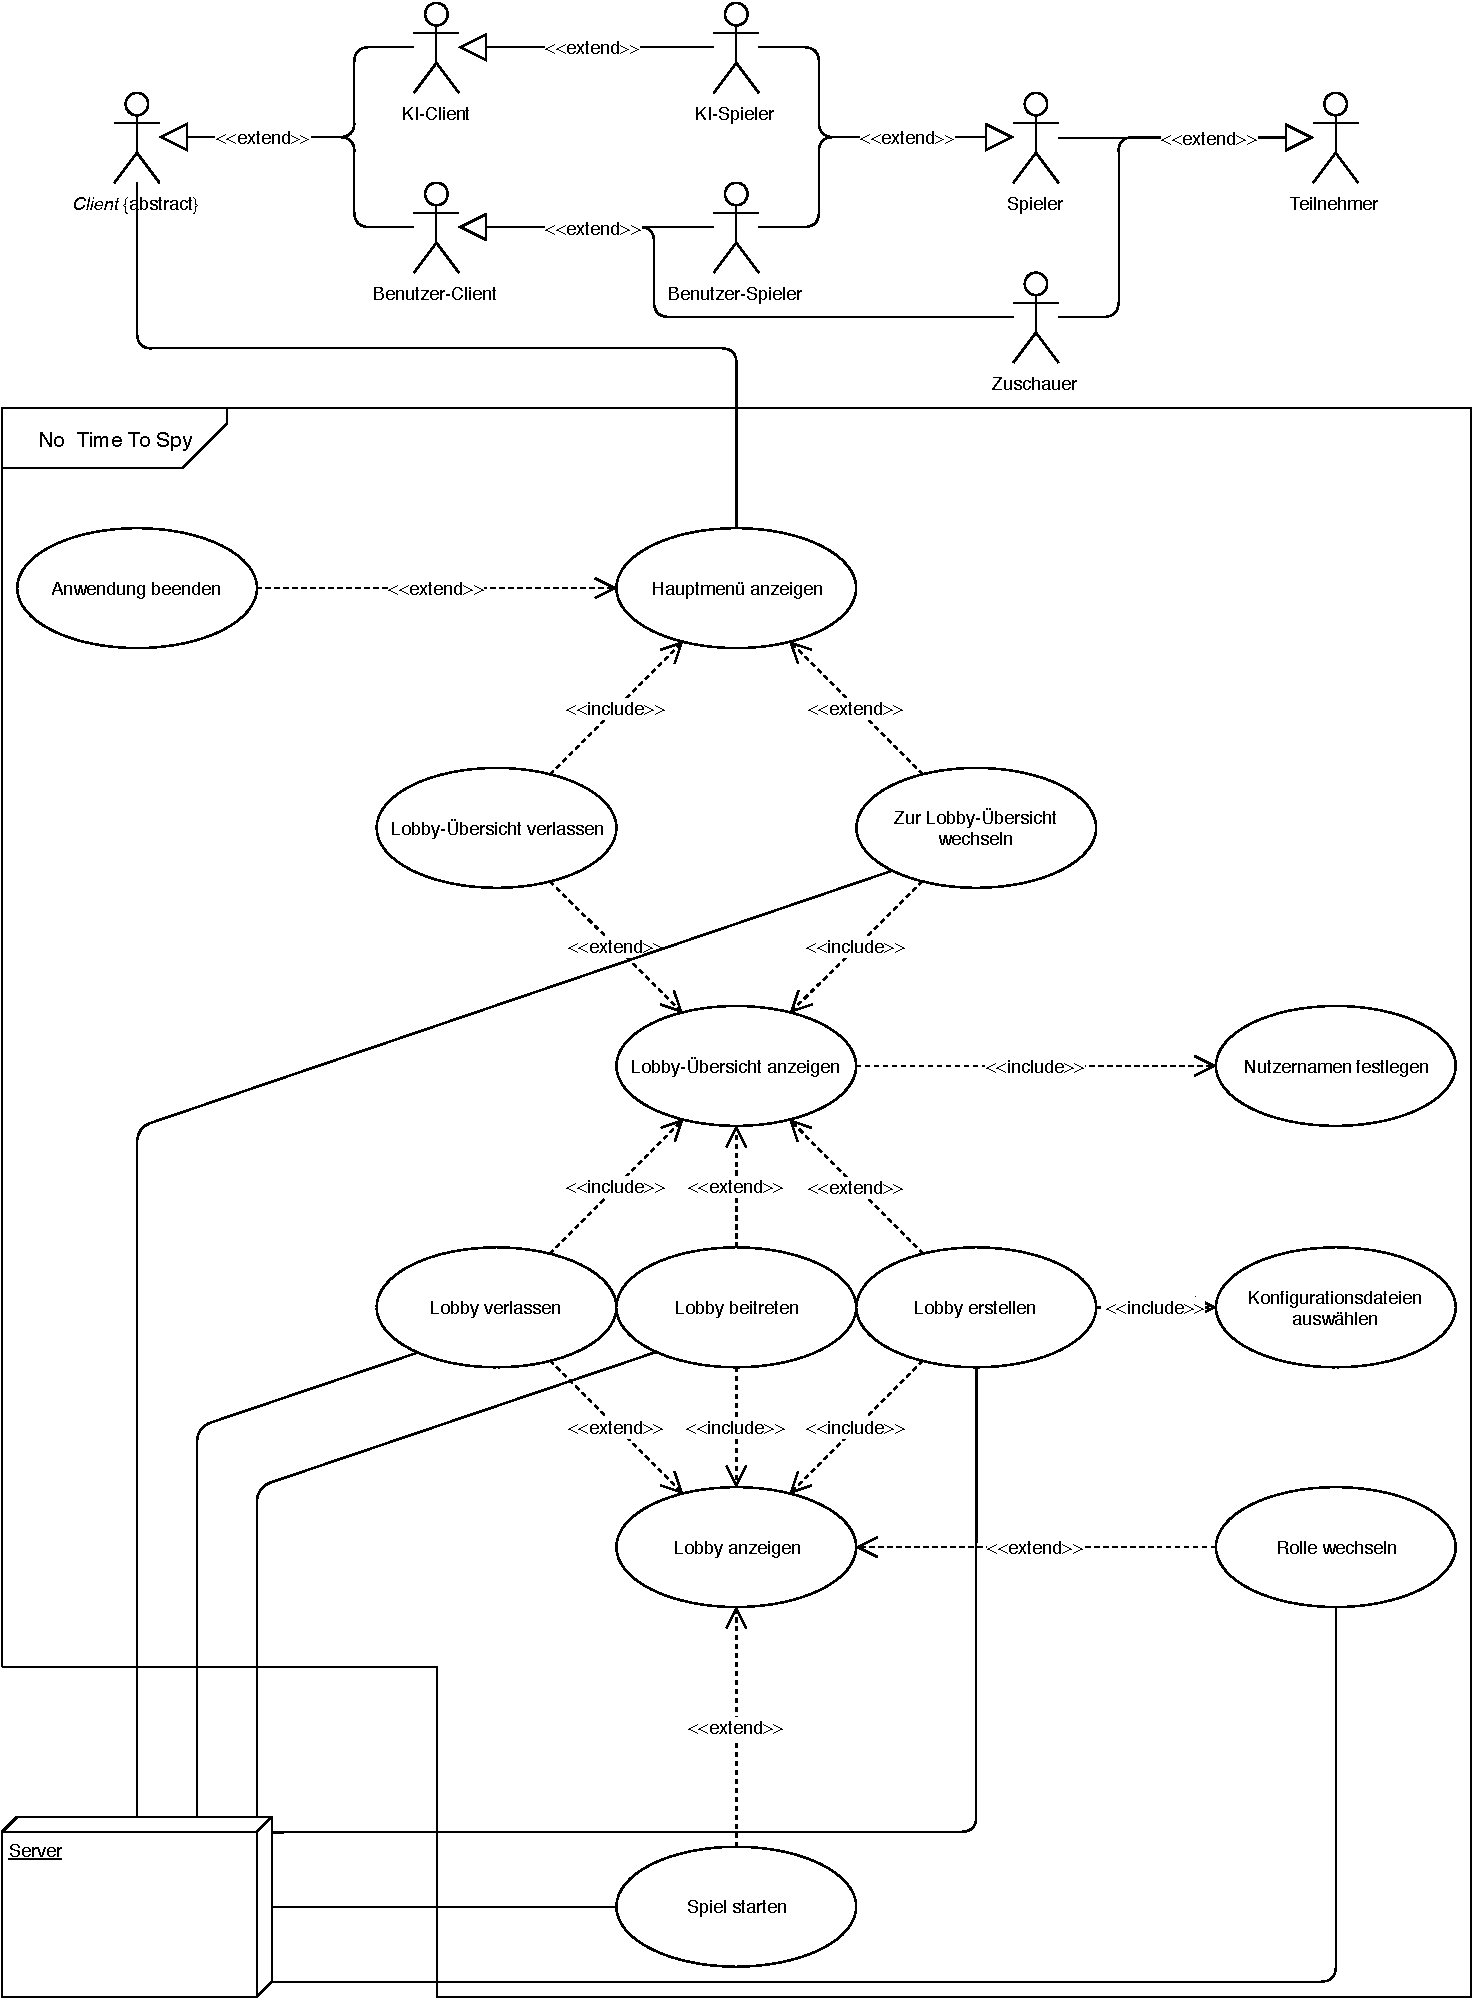
\includegraphics[width=\textwidth]{Meilenstein02/use_case_lobbymanagement.pdf}
  \caption{Anwendungsfälle Lobbymanagement}
\end{figure}